\chapter{Literature Review}

Four factors and their relationship to labor force participation rates were frequently brought up in the literature. The contribution to labor force participation rates that will be examined in the literature include: health, social welfare programs, educational attainment, and marital status and childcare.

Beginning with health, some literature suggests a relationship between health, emotional well-being, and labor force participation across different demographic groups. Notably, about half of prime-age men who are not in the labor force report having serious health conditions, with many relying on pain medication, primarily prescription opioids. Meanwhile, labor force participation among women born after 1960 has stagnated, with those outside the workforce citing reasons beyond home responsibilities reporting emotional well-being at similar levels to those in the workforce. By contrast, prime age men outside the labor force, report less happiness (Krueger, 2018)\footnote{Alan B. Krueger, Brookings Papers on Economic Activity, Fall 2017}. Labor can be important to well being of individuals and may limit the effects of policies on labor force participation rate. Some literature counters this notion, and suggests that with an increase in Disability Insurance the labor force participation rate declines. Between 1984 and 2001, the number of non-elderly adults receiving Social Security Disability Insurance (DI) increased by 60\%, reaching 5.3 million beneficiaries, despite improvements in overall health. This growth is attributed to several factors: less stringent screening processes, a decreased demand for low-skilled workers, and an unexpected rise in the earnings replacement rate. There has also been an increase in the likelihood of labor force exit among displaced high school dropouts, which contributed to a reduction of approximately 0.5 percentage points in the measured U.S. unemployment rate. The study projects a further increase in DI receipt rates moving forward (Duggan, Autor, 2003)\footnote{Autor, David \& Duggan, Mark. (2003). The Rise In The Disability Rolls And The Decline In Unemployment. The Quarterly Journal of Economics. 118. 157-205. 10.1162/00335530360535171.} (Parsons, 1980)\footnote{Parsons, Donald O. ``The Decline in Male Labor Force Participation.'' Journal of Political Economy, vol. 88, no. 1, 1980, pp. 117--34. JSTOR, \href{http://www.jstor.org/stable/1830962}{http://www.jstor.org/stable/1830962}. Accessed 11 Nov. 2024.}. However, even though unemployment rate accounts for those actively seeking out work, many individuals may be still searching for employment but not counted.

In terms of the domestic sphere, internationally governmental policies have skewed labor force participation. In countries with more robust publicly funded childcare, such as Sweden, literature finds there to be higher levels of labor market activity of women with preschoolers even regardless of spousal income. (Gustafsson, Stafford, 1984)\footnote{Gustafsson, Siv, and Frank Stafford. ``Child Care Subsidies and Labor Supply in Sweden.'' The Journal of Human Resources, vol. 27, no. 1, 1992, pp. 204--30. JSTOR, \cite{Gustafsson_1992}. Accessed 11 Nov. 2024.} While in West Germany, responses of surveys to mothers found that ``part-time working mothers would work full-time if they had greater access to subsidized child care'' (Bick, 2016)\footnote{Bick, Alexander. ``THE QUANTITATIVE ROLE OF CHILD CARE FOR FEMALE LABOR FORCE PARTICIPATION AND FERTILITY.'' Journal of the European Economic Association, vol. 14, no. 3, 2016, pp. 639--68. JSTOR, \href{http://www.jstor.org/stable/43965320}{http://www.jstor.org/stable/43965320}. Accessed 11 Nov. 2024.}. The pattern of a positive correlation between female labour force participation and childcare provision was found in cross-country analysis as well, with one study focusing on developed nations primarily in Europe, East Asia, and the United States (Borck, Rainald, Rabenmutter, 2014)\footnote{Borck, Rainald. ```Adieu Rabenmutter'---Culture, Fertility, Female Labour Supply, the Gender Wage Gap and Childcare.'' Journal of Population Economics, vol. 27, no. 3, 2014, pp. 739--65. JSTOR, \href{http://www.jstor.org/stable/44289682}{http://www.jstor.org/stable/44289682}. Accessed 11 Nov. 2024.}. Fertility and the linkage with economic activities and female labor force participation has also been argued to not be as pronounced nowadays as believed (Ashraf, 2013)\footnote{Ashraf, Quamrul H., et al. ``The Effect of Fertility Reduction on Economic Growth.'' Population and Development Review, vol. 39, no. 1, 2013, pp. 97--130. JSTOR, \href{http://www.jstor.org/stable/41811954}{http://www.jstor.org/stable/41811954}. Accessed 11 Nov. 2024.}. Similarly, expansion of welfare programs have been seen to increase the rate of female labor force participation. One paper explores the relationship between labor supply and the risk of divorce, suggesting that labor force participation might be influenced by marital stability (Johnson, Skinner, 1986)\footnote{Johnson, William R., and Jonathan Skinner. ``Labor Supply and Marital Separation.'' The American Economic Review, vol. 76, no. 3, 1986, pp. 455--69. JSTOR, \href{http://www.jstor.org/stable/1813362}{http://www.jstor.org/stable/1813362}. Accessed 11 Nov. 2024.}. Meanwhile the increase in participation of single mothers in the labor force ``most likely reflects the impact of the 1996 welfare reform act, in which the welfare entitlements embodied in the old Aid for Families with Dependent Children (AFDC) program were transformed into more temporary and conditional assistance in the Temporary Assistance to Needy Families (TANF) program'' (Juhn, Potter, 2006)\footnote{Juhn, Chinhui, and Simon Potter. ``Changes in Labor Force Participation in the United States.'' The Journal of Economic Perspectives, vol. 20, no. 3, 2006, pp. 27--46. JSTOR, \href{http://www.jstor.org/stable/30033665}{http://www.jstor.org/stable/30033665}. Accessed 11 Nov. 2024.}. The study's results indicate that female labor supply significantly increases after marital separation, while male labor supply sees a slight decline. Women often enhance their labor participation even before separation occurs, suggesting that anticipating divorce may drive them to work more. These findings highlight the influence of marital status on labor supply decisions, with women's labor force participation rising in response to potential instability in their marriages. (Johnson, Skinner, 1986)\footnote{Johnson, William R., and Jonathan Skinner. ``Labor Supply and Marital Separation.'' The American Economic Review, vol. 76, no. 3, 1986, pp. 455--69. JSTOR, \href{http://www.jstor.org/stable/1813362}{http://www.jstor.org/stable/1813362}. Accessed 11 Nov. 2024.}. Juhn and Potter's study finds that the U.S. labor force participation rate, which rose steadily from the mid-1960s, slowed in the 1990s and declined by 1.5 percentage points from its peak in 2000 by 2005. Key findings include that married women's participation is unlikely to rise significantly, while low-income single mothers may increase their workforce presence due to the Earned Income Tax Credit. Employers might adopt flexible work policies to attract mothers and older workers, and changes in disability and Social Security rules could impact men's withdrawal from the labor market and encourage delayed retirement among older workers (Juhn, Potter, 2006)\footnote{Juhn, Chinhui, and Simon Potter. ``Changes in Labor Force Participation in the United States.'' The Journal of Economic Perspectives, vol. 20, no. 3, 2006, pp. 27--46. JSTOR, \href{http://www.jstor.org/stable/30033665}{http://www.jstor.org/stable/30033665}. Accessed 11 Nov. 2024.}.

A core issue with any assessment of one factor and labor force participation is the aging demographic. In one study analyzing educational attainment and the impact on labor force participation rates it was found that for European women educational attainment did have a significant impact on their participation in the labor force, but that was not immediately statistically clear for overall rates due to the impact of aging demographics (Loichinger, Elke, Prskawetz, 2017)\footnote{Loichinger, Elke, and Alexia Prskawetz. ``Changes in Economic Activity: The Role of Age and Education.'' Demographic Research, vol. 36, 2017, pp. 1185--208. JSTOR, \href{http://www.jstor.org/stable/26332163}{http://www.jstor.org/stable/26332163}. Accessed 11 Nov. 2024.}. Isolation of variables may present difficulties when it comes to analysis of any one factor. Similarly, it was found that LFP rates of adult women and men in a study across European countries would have increased more during a period studied, 2000-2010, had it not been for the aging population (Loichinger, Prskawetz, 2017). \footnote{Loichinger, E., \& Prskawetz, A. (2017). Changes in economic activity: The role of age and education. Demographic Research, 36, 1185-1208. Max Planck Institute for Demographic Research.}

Together, several studies suggest there is a relationship between provisions of childcare by the state as it frees up the time for the mother and the entry of women into the labor force. Meanwhile, disability insurance and social security provisions have been suggested to de-incentivize entry into the labor force. Dependent upon the type of welfare will impact the affect on the labor force participation rate, however since childcare provisions aren't common in the U.S. democratic policies providing welfare will likely lead to lower labor force participation. Notably however, it is difficult to isolate any individual factor without the consideration of age.

Age is a significant factor and can be used to explain historical shifts in national participation rates. The steady rise in participation rates from 1948, after World War II through 2000 is due to the greater entry of women into the work force. In this chart, the US Bureau of Labor Statistics displays the shift in share of the labor force occupied by men versus women (U.S. Bureau of Labor Statistics, 2021).\footnote{U.S. Bureau of Labor Statistics. (2021, March 30). Celebrating Women's History Month with a look at women in the labor force. \href{https://www.bls.gov/blog/2021/celebrating-women-s-history-month-with-a-look-at-women-in-the-labor-force.htm}{https://www.bls.gov/blog/2021/celebrating-women-s-history-month-with-a-look-at-women-in-the-labor-force.htm}}

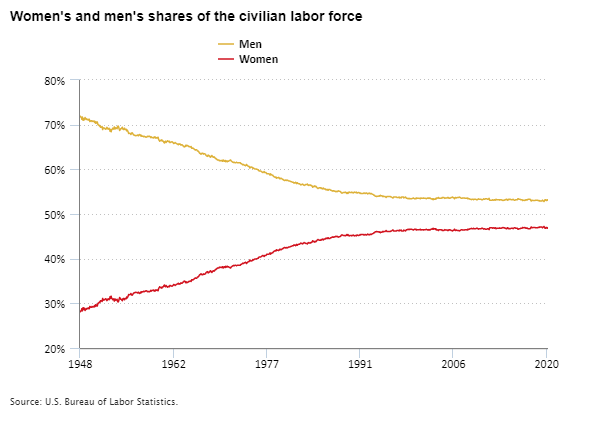
\includegraphics[width=0.7\linewidth]{files/women-73c868b7c60b99ec32c4060e9621d3c8.png}

Following the flattening of the labor force in the 1990s, the 2000s saw a decline, however that was not universal among all demographics. While rates fell for teenagers and young adults, rates increased for men and women over 55 (U.S. Bureau of Labor Statistics, 2016).\footnote{U.S. Bureau of Labor Statistics. (2016, September). Labor force participation: What has happened since the peak? Monthly Labor Review. \href{https://www.bls.gov/opub/mlr/2016/article/labor-force-participation-what-has-happened-since-the-peak.htm}{https://www.bls.gov/opub/mlr/2016/article/labor-force-participation-what-has-happened-since-the-peak.htm}}

Political party leadership may be an area of interest to observe as a large part of the reason those over 55 have began entering the workforce is connected to government instituted programs, namely Social Security. This is in addition to factors such as changes to private retirement plans, an aging population, rising health care costs, and increase in educational attainment (Leonesio, Bridges, Gesumaria, \& Del Bene, 2010).\footnote{Leonesio, M. V., Bridges, B., Gesumaria, R., \& Del Bene, L. (2010, August 22--28). The increasing labor force participation of older workers and its effect on the income of the aged. Social Security Bulletin, 72(1), 59--70. \href{https://www.ssa.gov/policy/docs/ssb/v72n1/v72n1p59.html}{https://www.ssa.gov/policy/docs/ssb/v72n1/v72n1p59.html}}

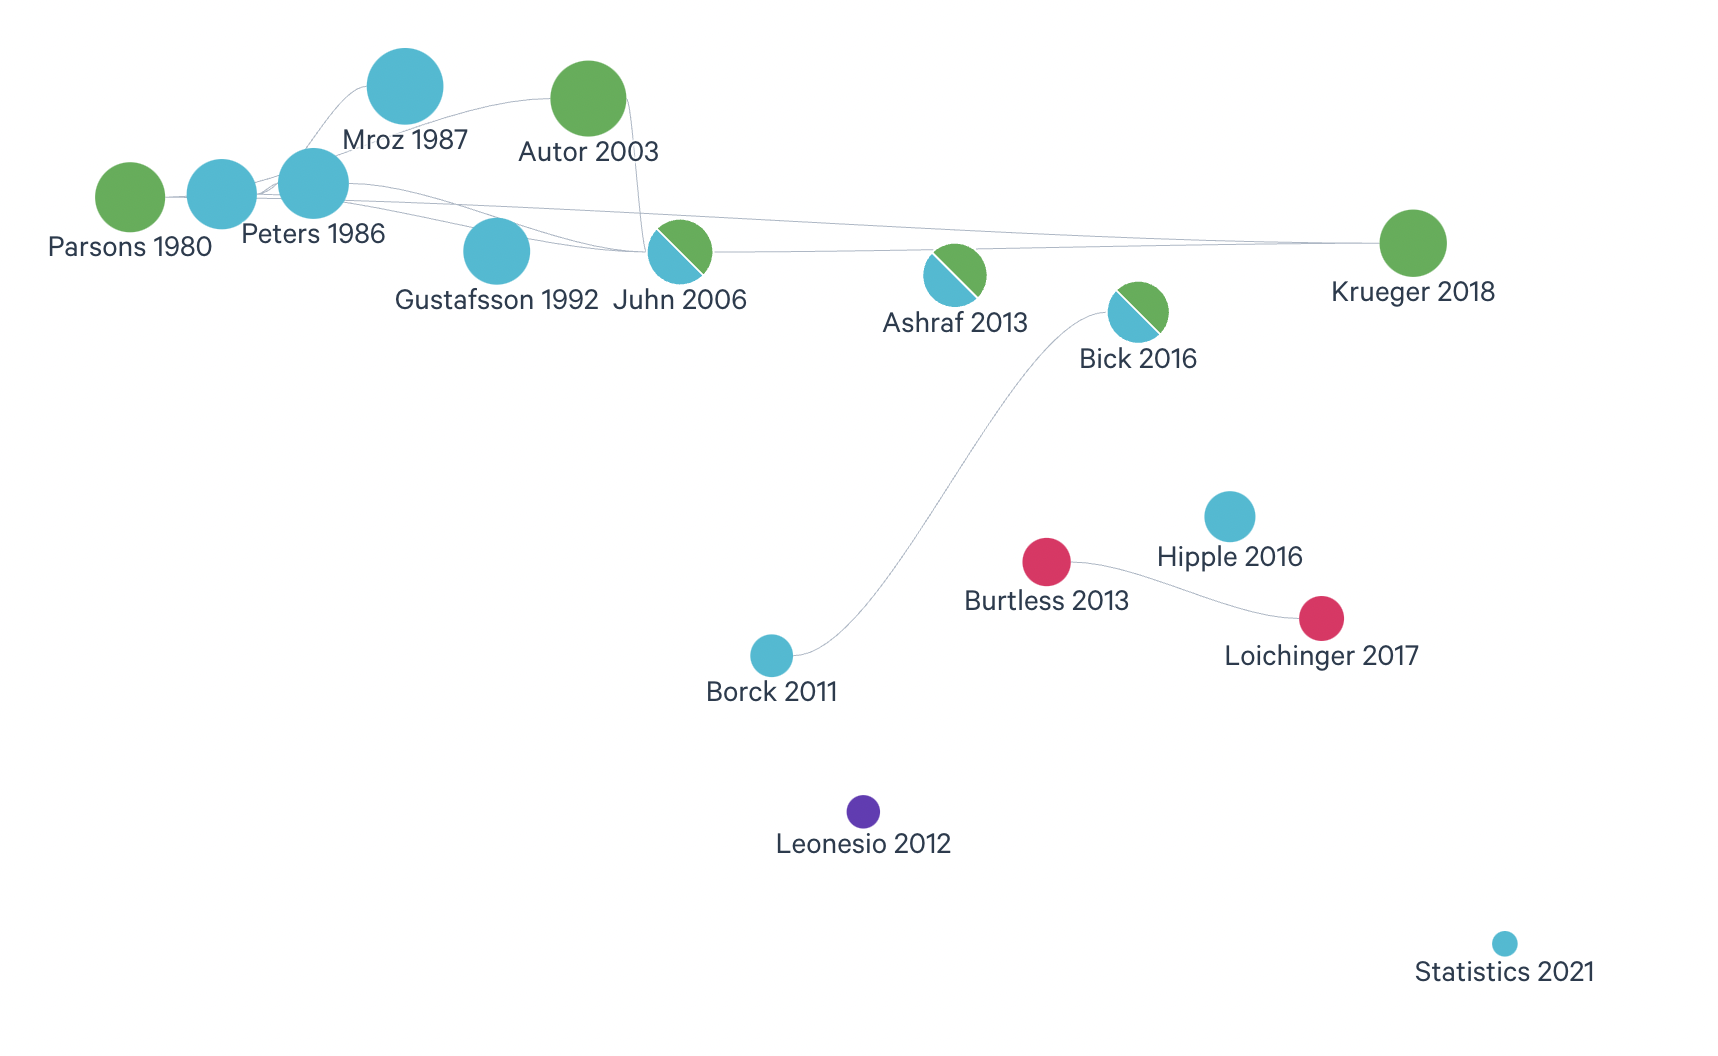
\includegraphics[width=0.7\linewidth]{files/litmap-ba9102f2e95757a03bd4124d2527438a.png}

Access Litmap here\footnote{\href{https://app.litmaps.com/shared/27382733-b5c6-486d-a482-e2b972a348ed}{https://app.litmaps.com/shared/27382733-b5c6-486d-a482-e2b972a348ed}}